\chapter{Sampling via transformation of coordinates}

\section{Sampling uniformly within a unit radius disk}\label{ex:021}

\begin{sourcefiles}
  \item[Source codes] src/021\_disk\_sampling.c
  \item[Analysis scripts] src/021\_disk\_sampling.R
  \item[Executables] exe/021\_disk\_sampling
\end{sourcefiles} 

If we want to sample points uniformly distributed over the unit disk, we cannot
simply generate $r \sim \unif{0}{1}$ and $\theta \sim \unif{0}{2\pi}$. The
result of doing that is shown in the left graph of \figref{fig:021}. While the
angular distribution poses no problem, there is an undesired higher density of
points close to the centre of the disk.

\begin{figure}
  \centering
  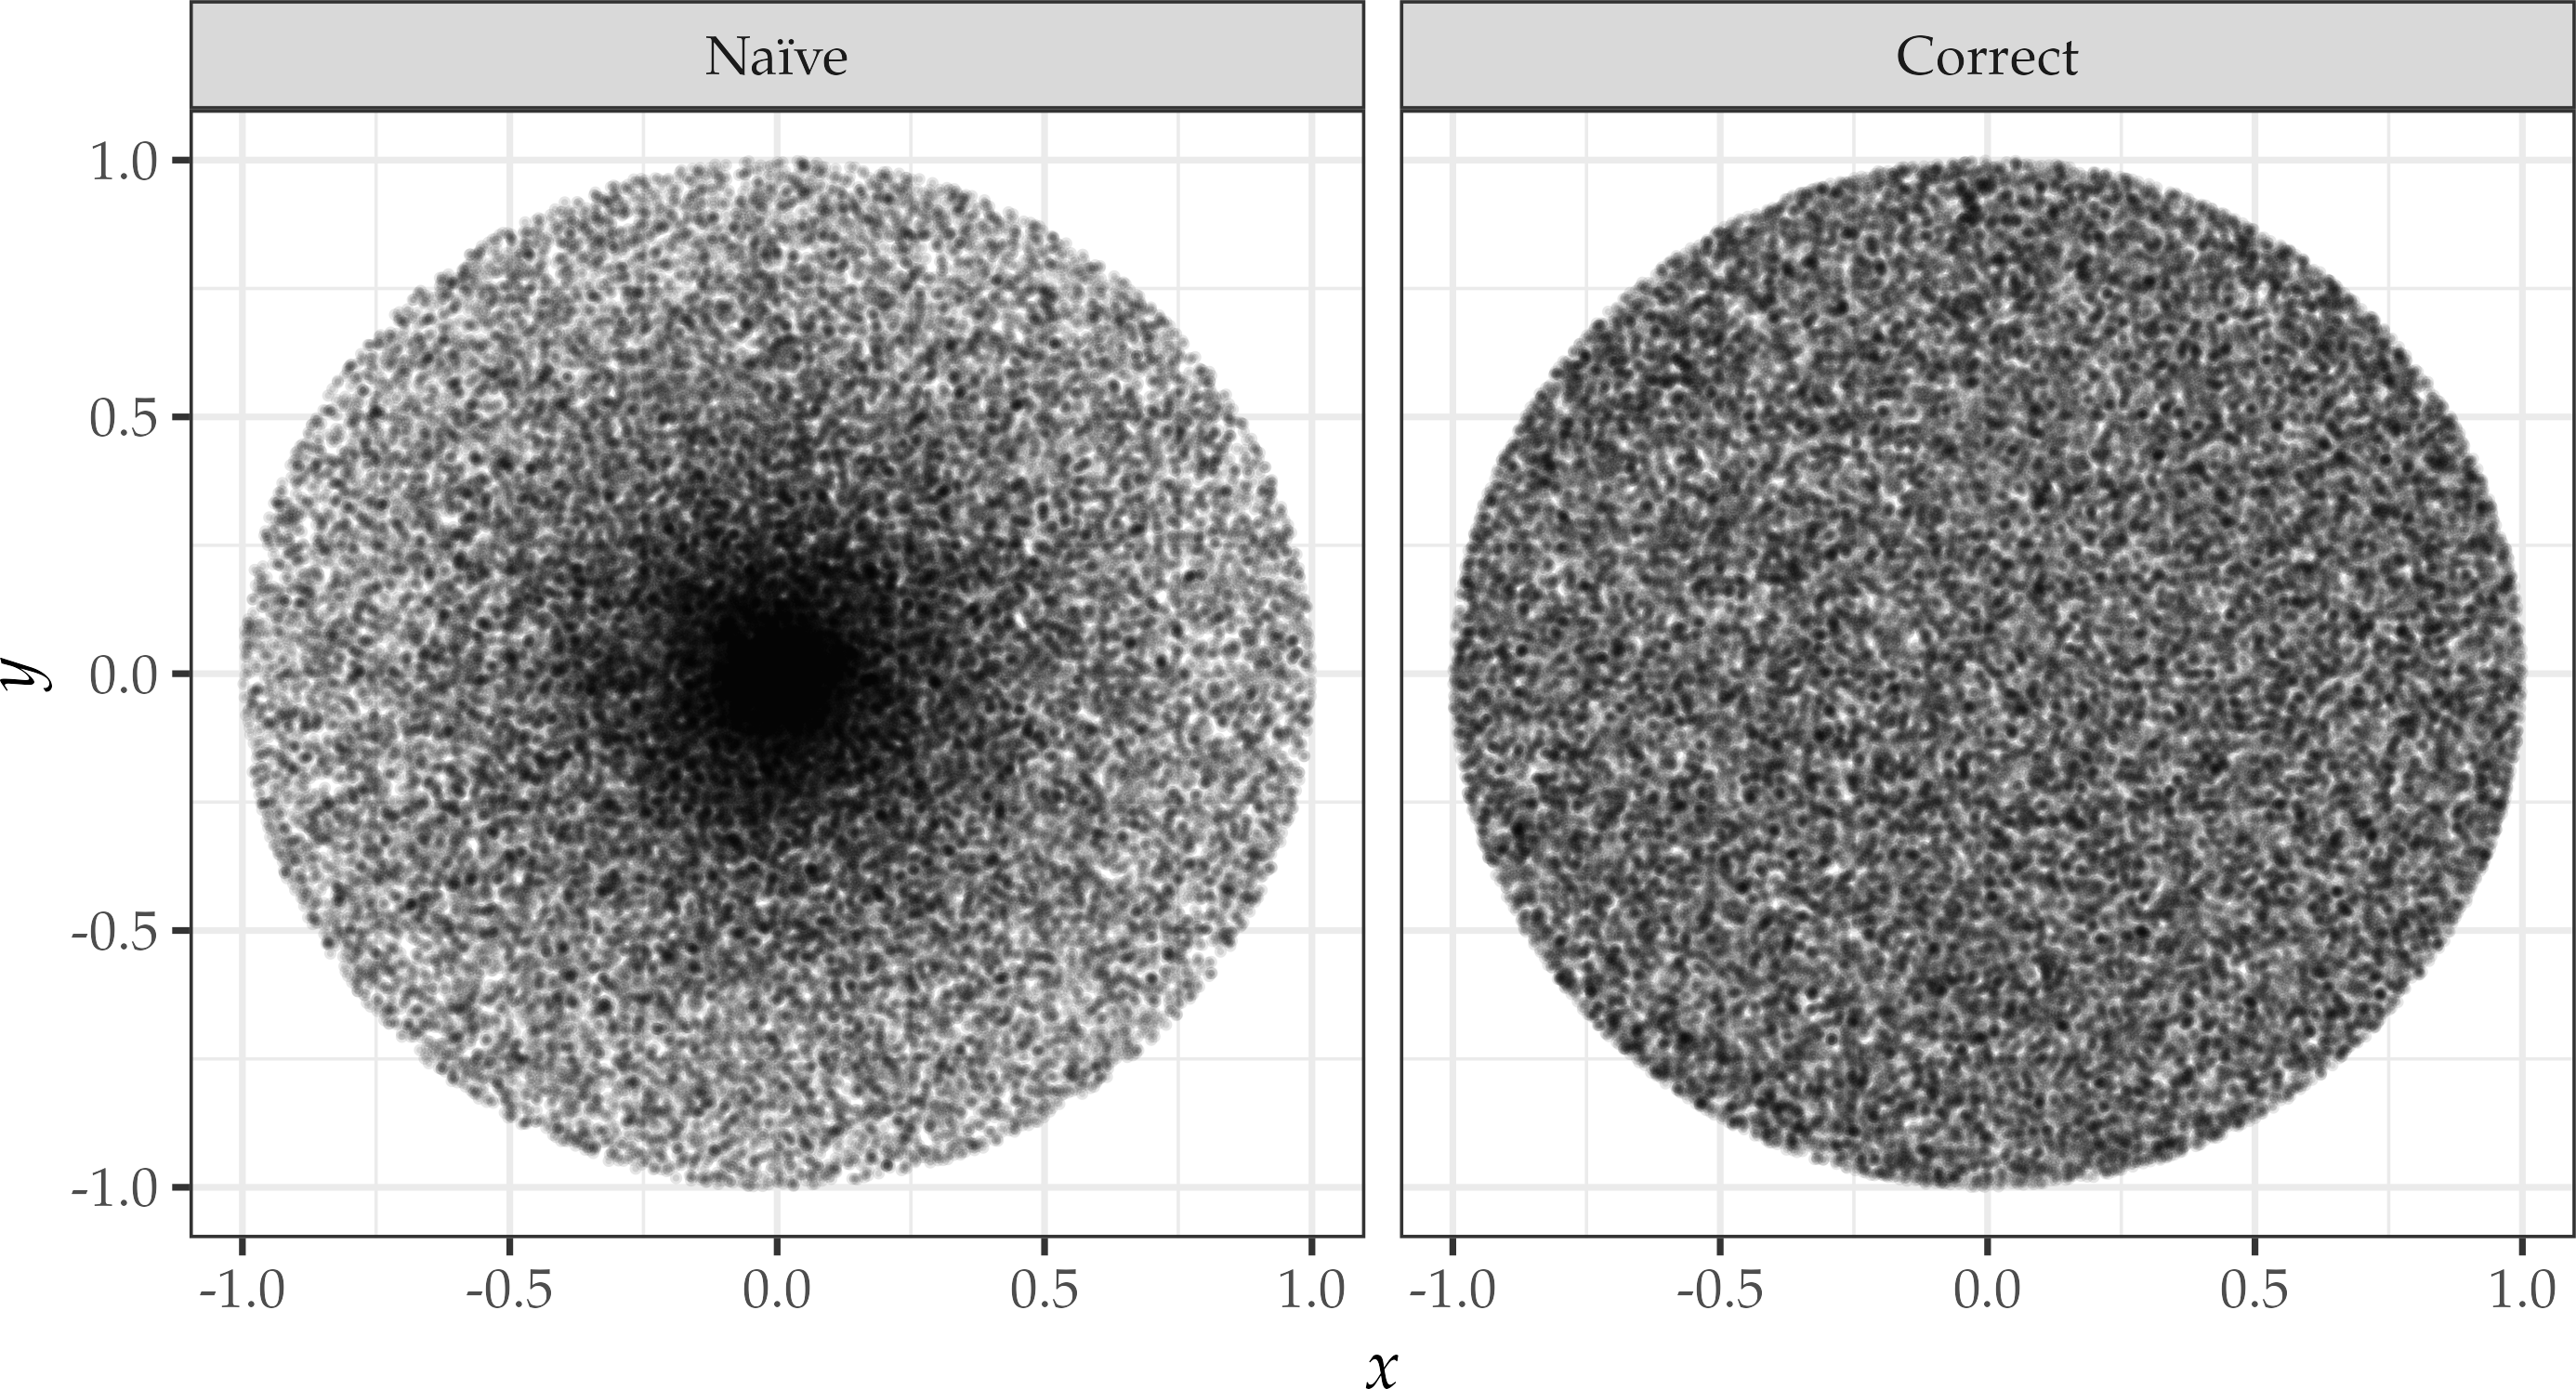
\includegraphics{img/021.png}
  \caption{visualization of \num{50000} samples on the unit disk, with the
    \enquote{naïve} method of uniform sampling both on $r$ and $\theta$
    (left), and with the correct method described in the text (right).}
  \label{fig:021}
\end{figure}

The reason for this becomes clear when you consider the number of points falling
inside a ring of given thickness $\delta r$. Consider a ring with inner radius
$r_1$ and outer radius $r_1 + \delta r$, with $\delta r \ll r_1$, and another
with radii $r_2$, $r_2 + \delta r$.  Despite the ratio of their areas being
\begin{equation}
  \frac{\cancel{\pi} \left[(r_{1} + \delta r)^{2} -
  r_{1}^{2}\right]}{\cancel{\pi} \left[(r_{2} + \delta r)^{2} -
  r_{2}^{2}\right]} = \frac{2r_{1} \delta r + \bigo{\delta r^{2}}}{2 r_{2}
  \delta r + \bigo{\delta r^{2}}} = \frac{r_{1}}{r_{2}} + \bigo{\delta r},
\end{equation}
the fraction of points within each ring is in both cases proportional to $\delta
r$, if $r$ is sampled uniformly. Thus, the number of points falling at a
distance $r$ should be proportional to $r$:
\begin{equation}
  \rho_{r}(r) = 2r,
\end{equation}
with the $2$ in front to ensure normalization over $[0, 1]$. By computing the
cumulative and inverting we get 
\begin{equation}
  F_r(r) = 2 \int_{0}^{x} x \, dx = x^{2} \implies u = r^{2} \implies r =
  \sqrt{u}.
\end{equation}
The graph on the right in \figref{fig:021} shows how the sampling becomes
visibly uniform with this adjustment.

\section{Box--Muller transform}\label{ex:022}

\begin{sourcefiles}
  \item[Source codes] src/022\_box\_muller.c
  \item[Analysis scripts] src/022\_box\_muller.R
  \item[Executables] exe/022\_box\_muller
\end{sourcefiles} 

I started from the factorization of $\rho_{x, y}(x, y)$:
\begin{equation}
  \rho_{x, y}(x, y) = \frac{1}{2\pi} \exp\left(-\frac{x^{2} + y^{2}}{2}\right) =
  \rho_x(x) \rho_y(y), \quad \text{with } \rho_x(x) =
  \frac{e^{-x^{2}/2}}{\sqrt{2\pi}}.
\end{equation}
If we switch to polar coordinates this becomes, remembering the factor $r$
coming from the Jacobian,
\begin{equation}
  \rho_{r, \theta}(r, \theta) = \frac{r}{2\pi} e^{-r^{2}/2},
\end{equation}
with $\rho_r(r) = r e^{-r^{2}/2}$ and $\rho_\theta(\theta) = 1 / 2\pi$.

Then, we can marginalize over $\theta$ to get $\rho_r(r)$:
\begin{equation}
  \rho_r(r) = \frac{1}{2\pi} \int_{0}^{2\pi} r e^{-r^{2}/2} \, dr = r
  e^{-r^{2}/2}.
\end{equation}
As usual, we compute the cumulative and invert it to generate a random $r \sim
\rho_r(r)$:
\begin{equation}
  F_r(r) = \int_{0}^{r} x e^{-x^{2}/2} \, dx = 1 - e^{-r^{2}/2} \implies
  e^{-r^{2}/2} = 1 - u \implies r = \sqrt{-2 \log(1 - u)}.
\end{equation}
Then, to get the angle $\theta$ we recover the \emph{conditional} distribution
$\rho_{\theta\given r}(\theta \given r)$:
\begin{equation}
  \rho_{\theta\given r}(\theta\given r) = \frac{\rho_{r, \theta}(r,
  \theta)}{\rho_{r}(r)} = \frac{1}{2\pi}.
\end{equation}
Thus, for $\theta$ we have simply to sample from $\unif{0}{2\pi}$.

The idea then is to sample two numbers $u_{1}, u_{2}$ from $\unif{0}{1}$ at each
iteration; at that point we can calculate
\begin{equation}
  x = \sqrt{-2\log u_1} \cos(2\pi u_2), \quad y = \sqrt{-2\log u_1} \sin(2\pi
  u_2),
\end{equation}
to get two numbers $x, y$ distributed according to a standard Gaussian
$\gaus{0}{1}$. We can also get a $z \sim \gaus{\mu}{\sigma^2}$ afterwards by
multiplying $x$ or $y$ by $\sigma$ and summing the mean: $z = \mu + \sigma x$. I
ran a simulation with \num{100000} samples choosing $\mu = 1$ and $\sigma = 2$,
and you can see the results in \figref{fig:022}.

\begin{figure}
  \centering
  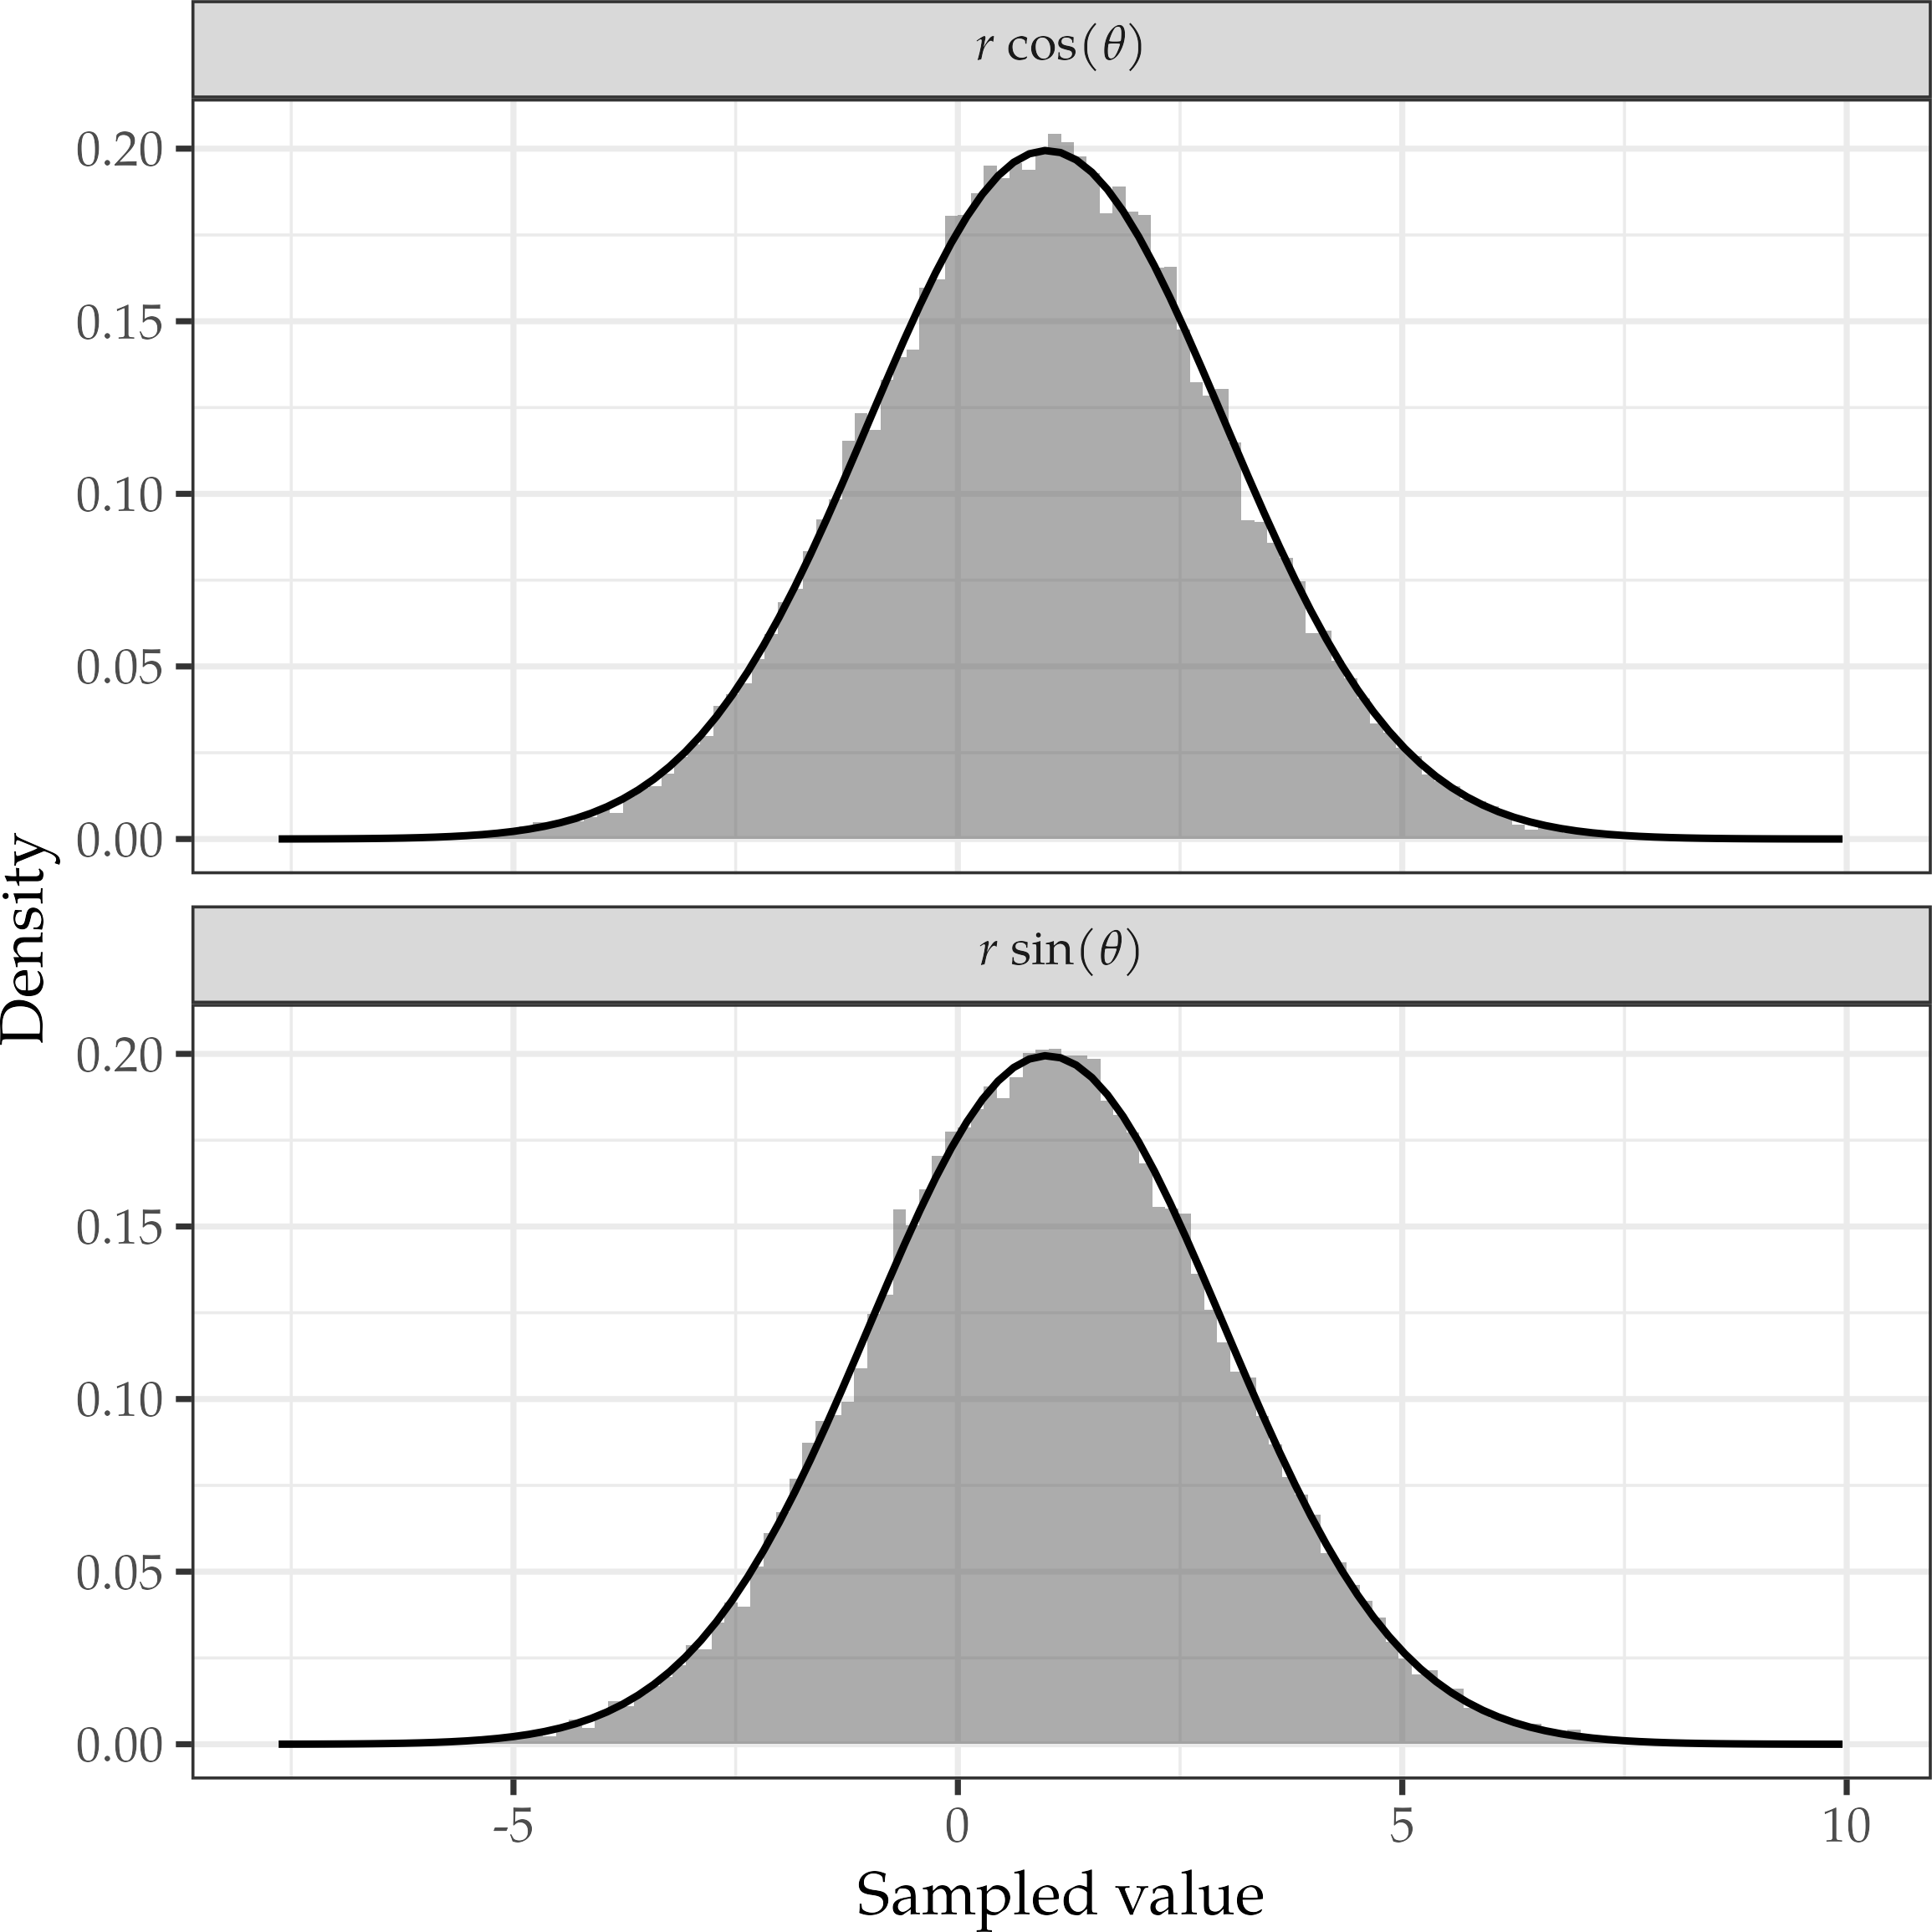
\includegraphics{img/022.png}
  \caption{histograms of \num{100000} samples -- half in the upper panel, half in
    the lower one -- from a $\gaus{1}{4}$ distribution, obtained with the
    Box--Muller method. The theoretical distribution is overlaid with a solid
    line.}
  \label{fig:022}
\end{figure}

\section{Rejection method}\label{ex:023}

\begin{sourcefiles}
  \item[Source codes] src/023a\_rejection\_sampling.c,
    src/023b\_rejection\_accratio.c
  \item[Analysis scripts] src/023\_rejection\_method.R
  \item[Executables] exe/023a\_rejection\_sampling,
    exe/023b\_rejection\_accratio
\end{sourcefiles} 

Here I implemented the sampling of random numbers from the distribution $f(x) =
2 e^{-x^{2}} / \sqrt{\pi}$ over $[0, \infty)$. We start from a function $g(x)$
that could serve as an upper limit to $f(x)$,
\begin{equation}
  g(x) =
  \begin{dcases}
    A & \text{for } 0 \leq x \leq p, \\
    \frac{A}{p}x e^{p^{2} - x^{2}} & \text{for } x > p.
  \end{dcases}
\end{equation}
First we normalize it to turn it into a proper probability distribution:
\begin{equation}
  1 = \int_{0}^{\infty} g(x) \, dx = Ap + \frac{A}{p}e^{p^{2}} \int_{p}^{\infty}
  x e^{-x^{2}} \, dx = A \left(p + \frac{1}{2p}\right) \implies A = \frac{2p}{1
  + 2p^{2}}.
\end{equation}
Then we need a constant $c$ such that $c g(x) \geq f(x)$ everywhere. The maximum
of $f(x)$ is in $x = 0$, where $f(0) = 2 / \sqrt{\pi}$, so we set $c A = 2 /
\sqrt{\pi}$. Another thing to consider is that $g(x)$ can have a maximum larger
than $A$ in $[p, \infty)$:
\begin{equation}
  g'(x) = 
  \begin{dcases}
    0 & \text{for } 0 \leq x \leq p, \\
    \frac{A}{p}(1 - 2x^{2}) e^{p^{2} - x^{2}} & \text{for } x > p.
  \end{dcases}
\end{equation}
Thus in the region $[p, \infty)$ the derivative is zero in $x = 1 / \sqrt{2}$.
To avoid this we have to choose $p \geq 1 / \sqrt{2} \approx \num{0.707}$. An
example of sampling with $p = 1 / \sqrt{2}$ is given by the histogram in
\figref{fig:023a}. A plot of the acceptance ratio as a function of $p$, starting
from the minimum value $1 / \sqrt{2}$, is shown in \figref{fig:023b}; obviously
the acceptance ratio decreases as $p$ increases, as the gap between $cg(x)$ and
$f(x)$ grows wider:
\begin{equation}
  \begin{split}
    \int_{0}^{\infty} (cg(x) - f(x))\, dx
    &= \frac{2}{\sqrt{\pi}} \int_{0}^{p} dx + \frac{2}{p \sqrt{\pi}}
    \int_{p}^{\infty} x e^{p^{2} - x^{2}} \, dx - 1 \\
    &= \frac{2}{\sqrt{\pi}} \left(p + \frac{1}{2p}\right) - 1
    \xrightarrow{p \to \infty} \infty.
  \end{split}
\end{equation}

\begin{figure}
  \centering
  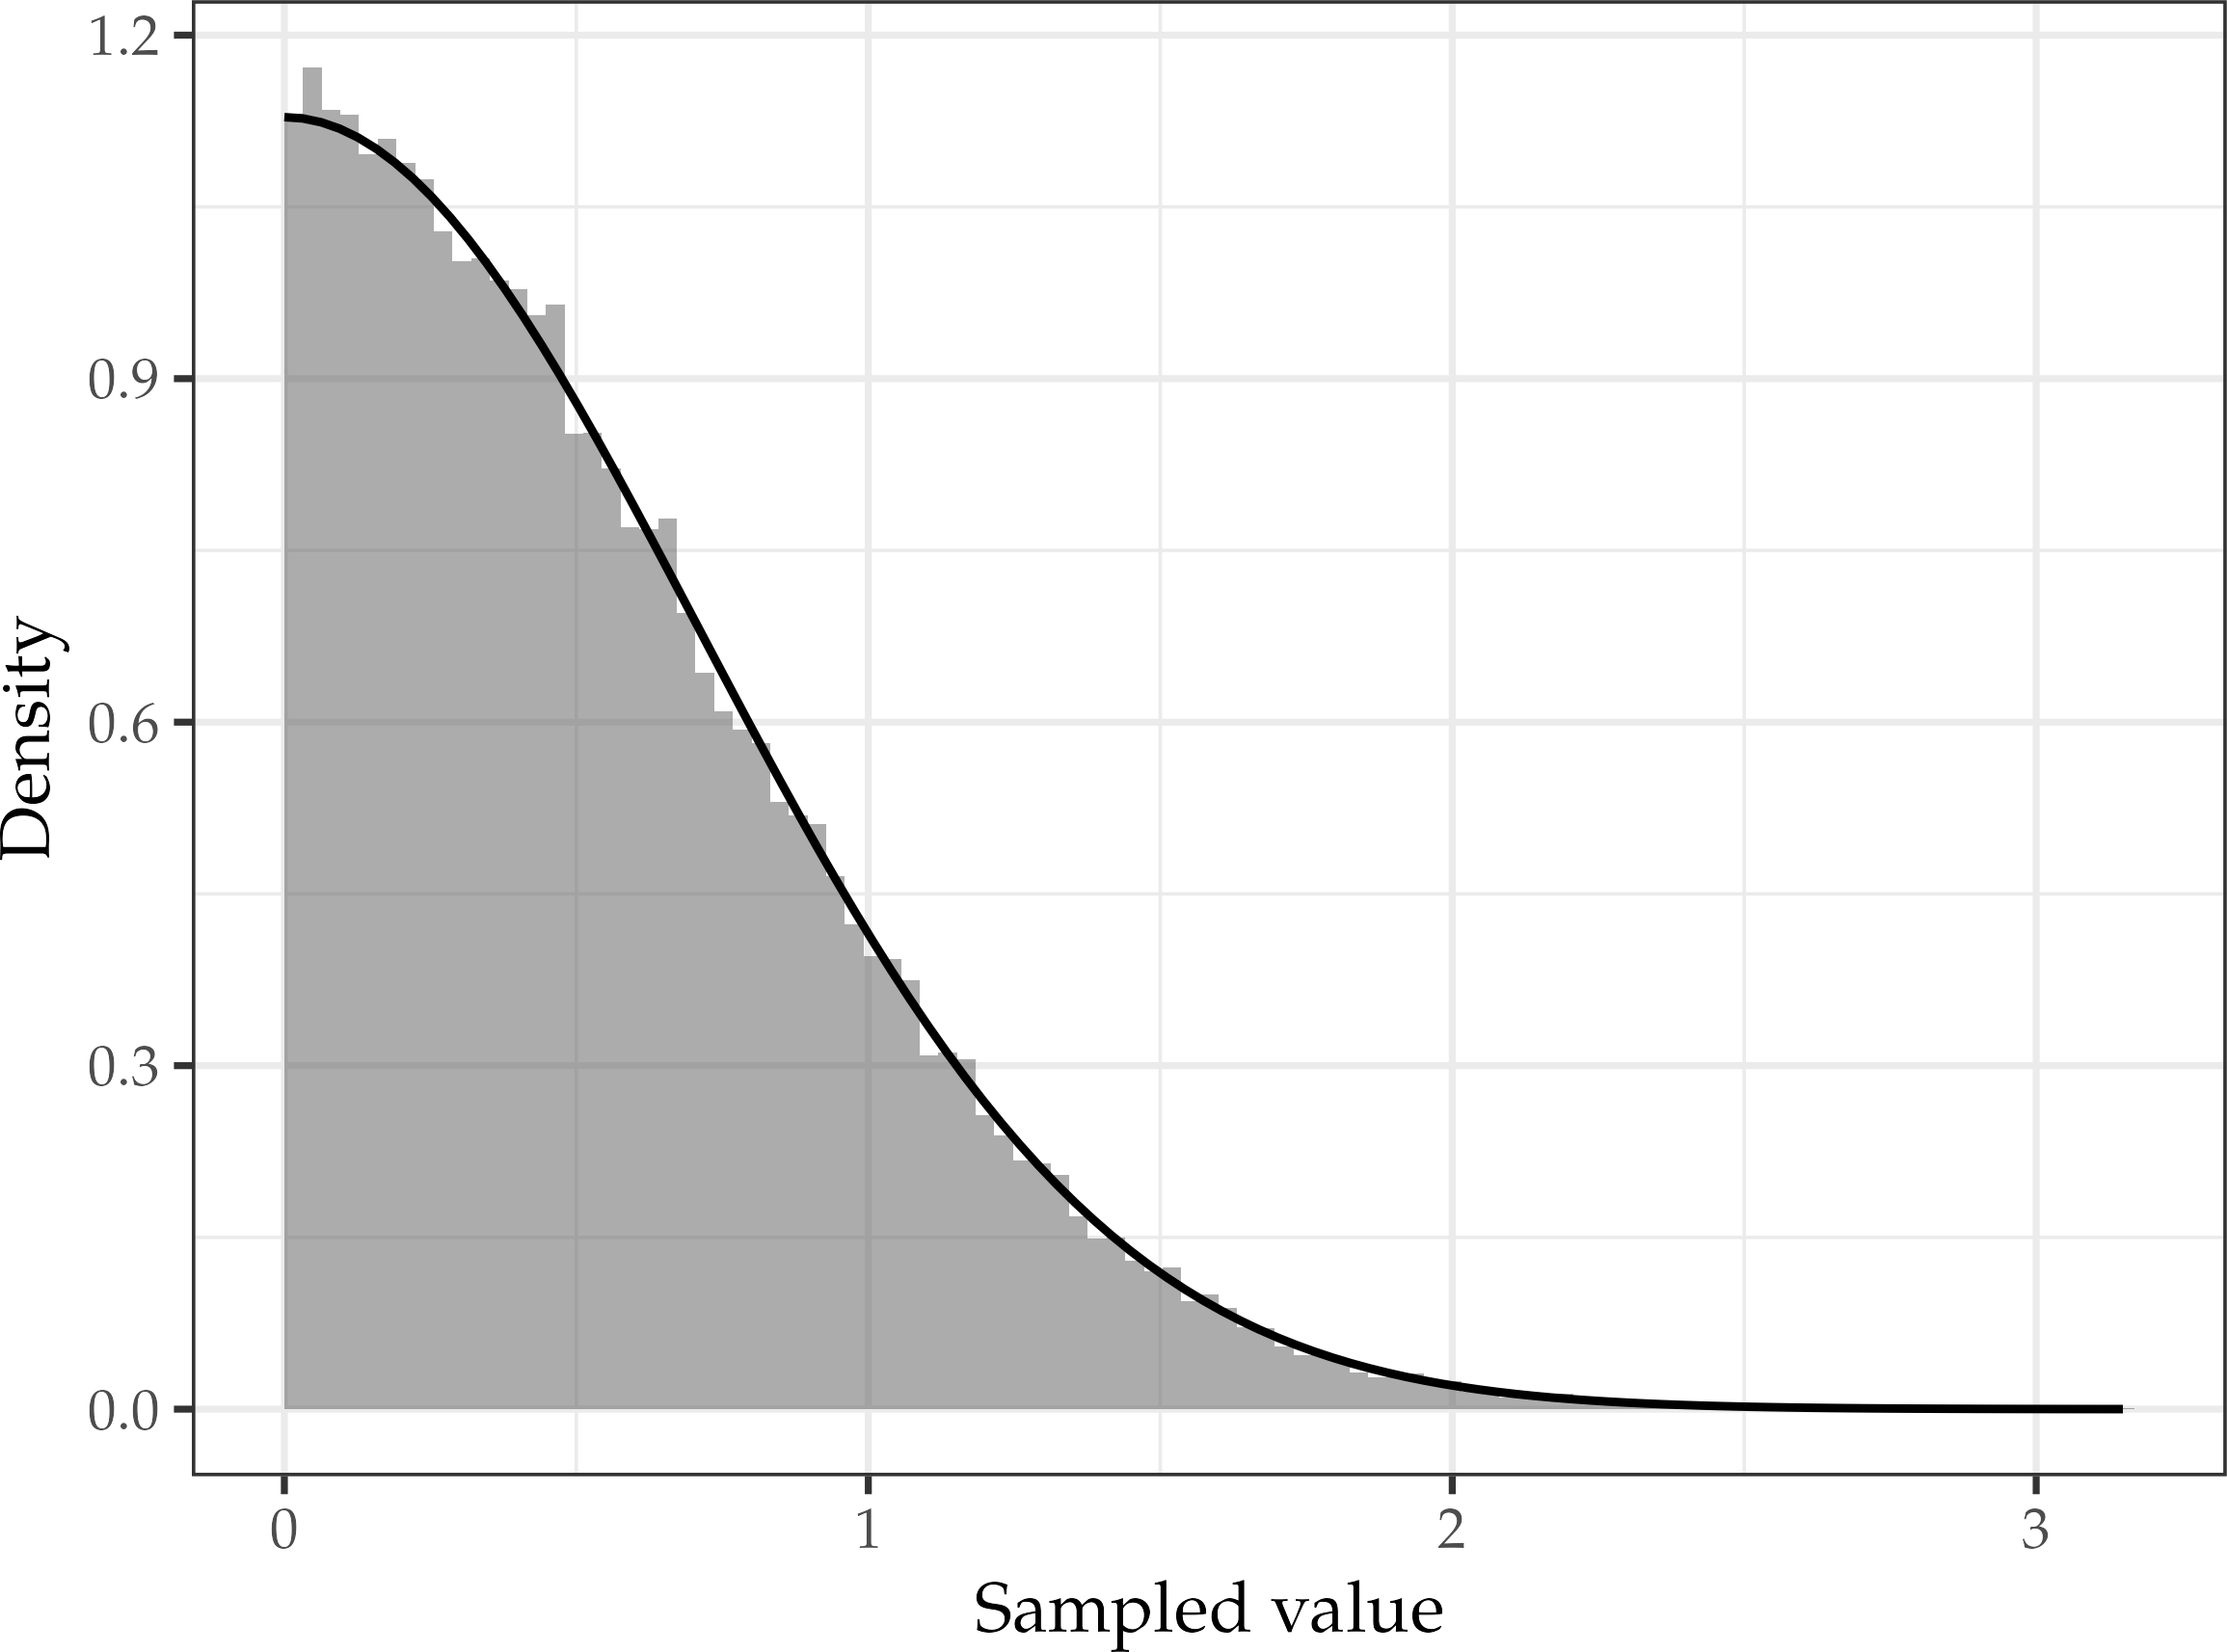
\includegraphics{img/023a.png}
  \caption{histogram of \num{50000} samples from the distribution $f(x) = 2
    e^{-x^{2}} / \sqrt{\pi}$ in $[0, \infty)$ obtained with the rejection
    method. The theoretical distribution is overlaid with a solid line.}
  \label{fig:023a}
\end{figure}

\begin{figure}
  \centering
  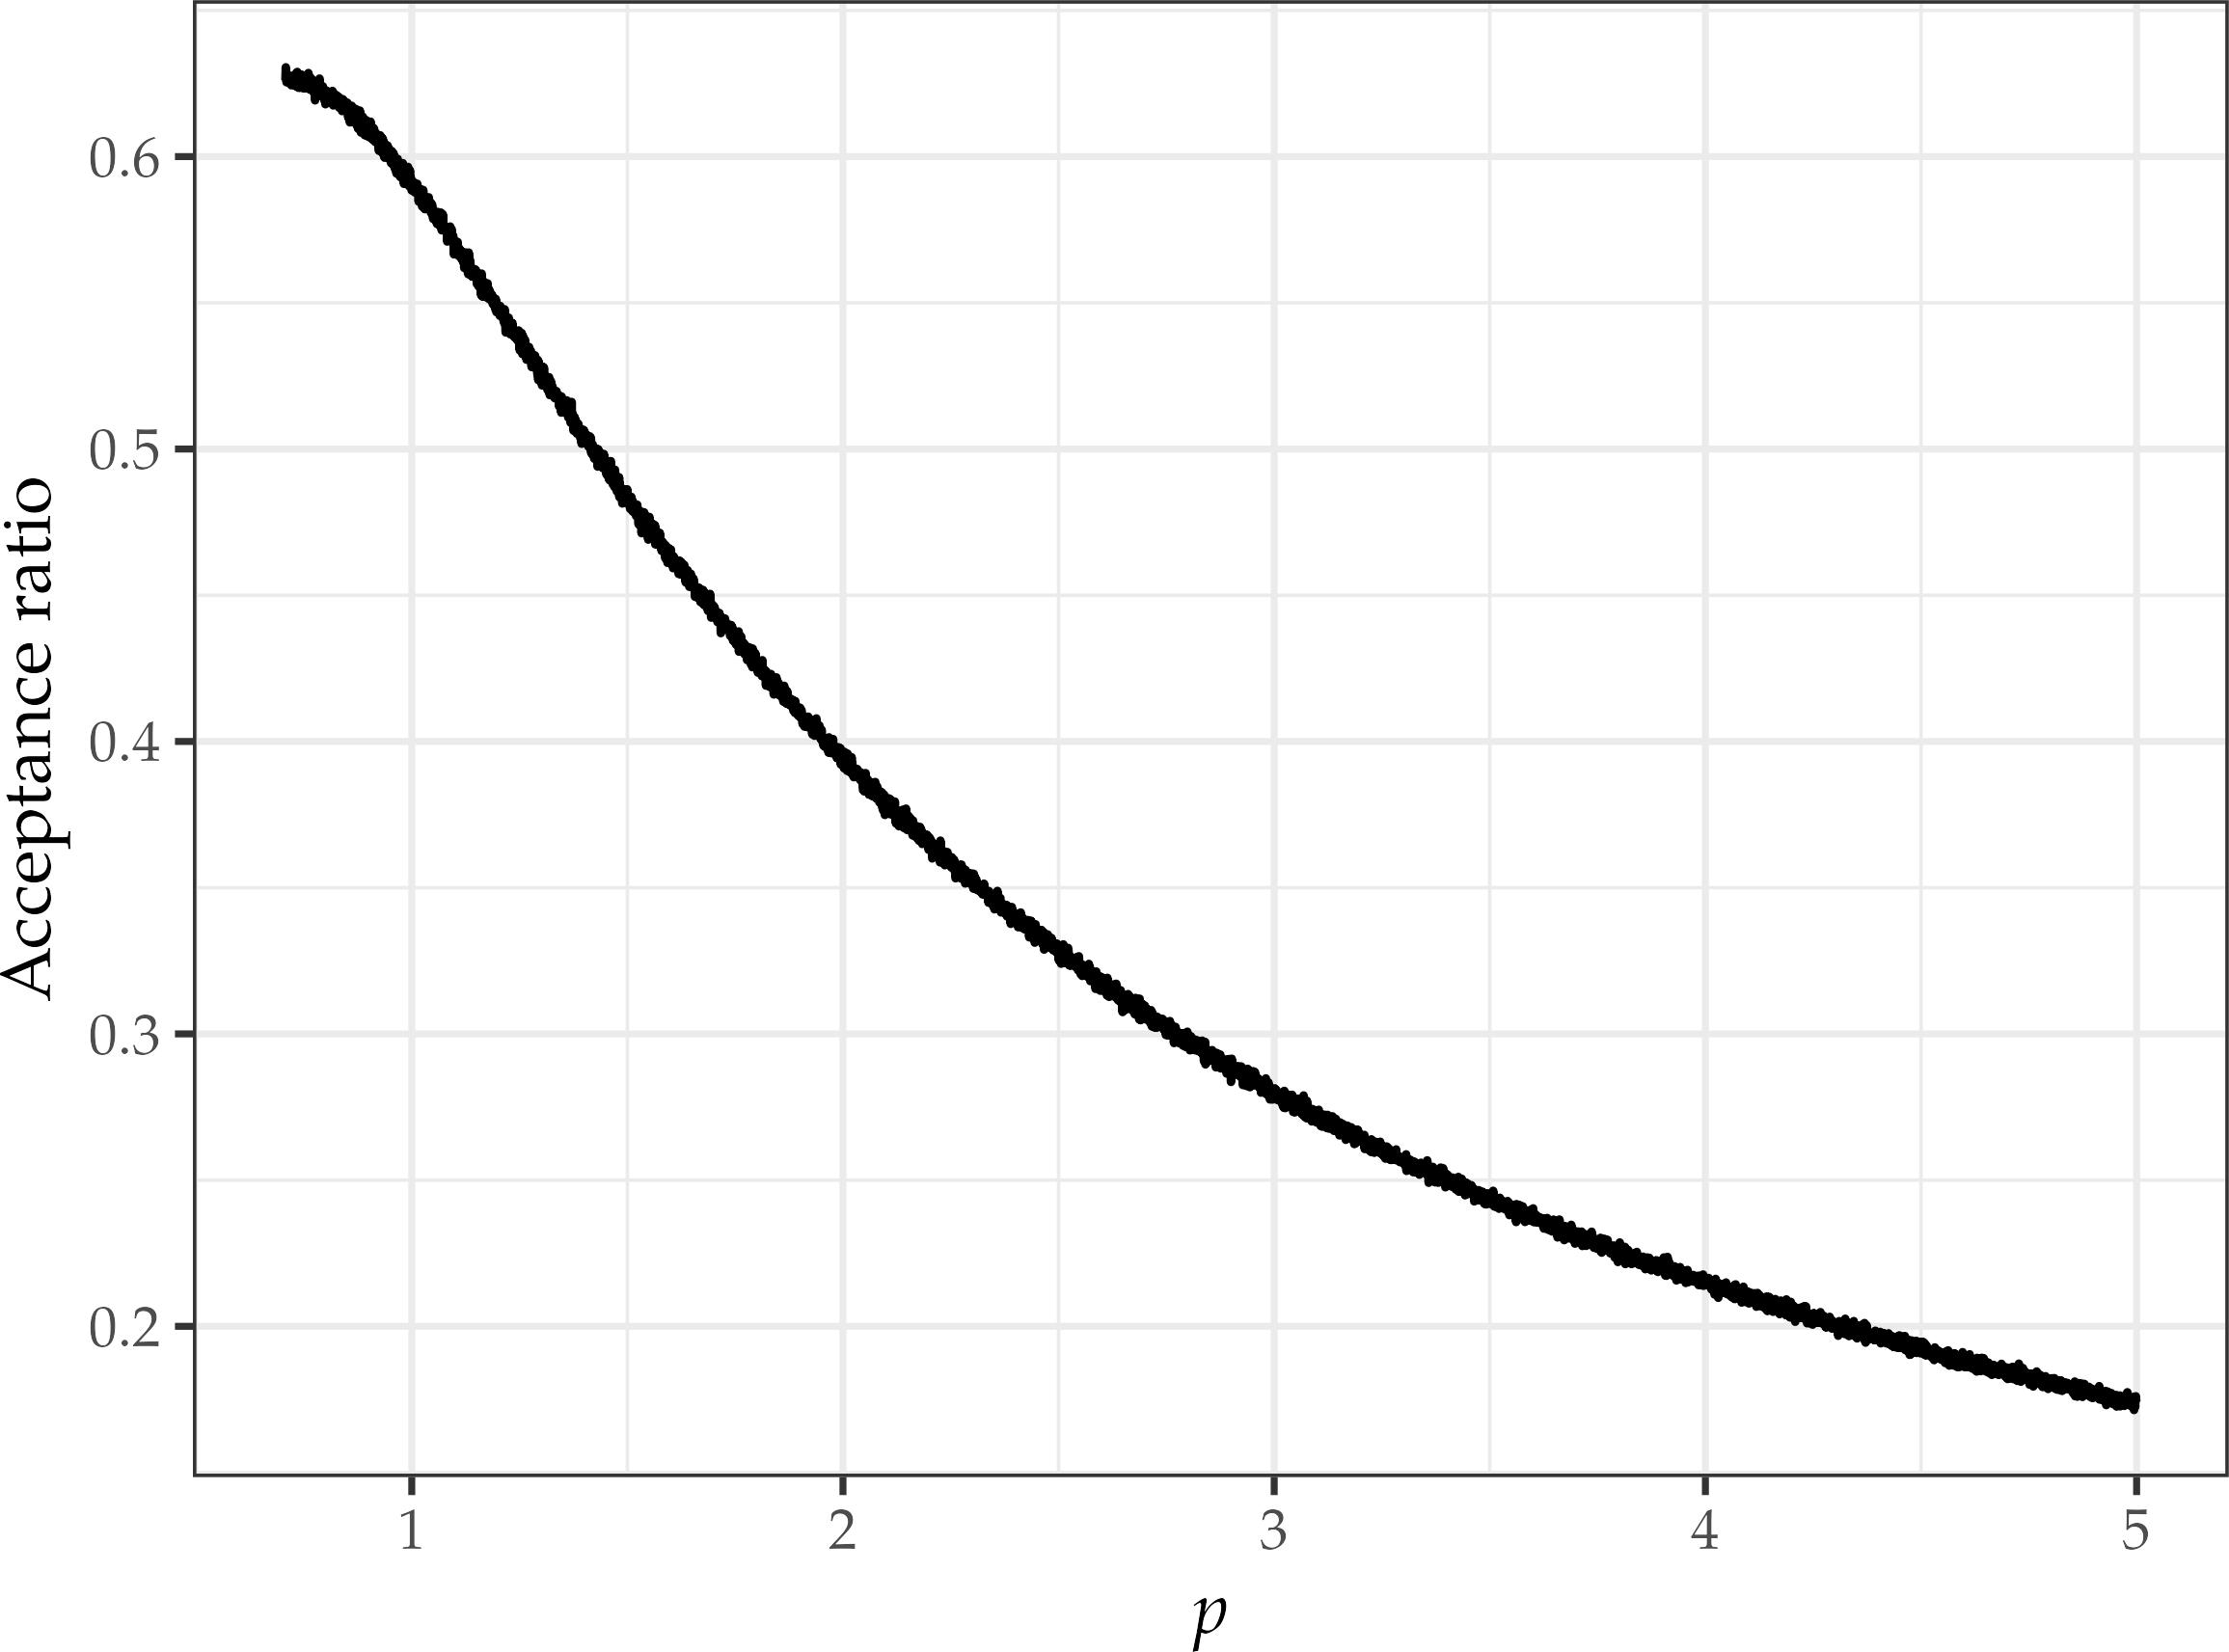
\includegraphics{img/023b.png}
  \caption{acceptance ratio over \num{100000} samples as a function of $p$ in
    \exref{ex:023}.}
  \label{fig:023b}
\end{figure}
